\documentclass[paper=letter,11pt]{scrartcl}

\KOMAoptions{headinclude=true, footinclude=false}
\KOMAoptions{DIV=14, BCOR=5mm}
\KOMAoptions{numbers=noendperiod}
\KOMAoptions{parskip=half}
\addtokomafont{disposition}{\rmfamily}
\addtokomafont{part}{\LARGE}
\addtokomafont{descriptionlabel}{\rmfamily}
%\setkomafont{pageheadfoot}{\normalsize\sffamily}
\setkomafont{pagehead}{\normalsize\rmfamily}
%\setkomafont{publishers}{\normalsize\rmfamily}
\setkomafont{caption}{\normalfont\small}
\setcapindent{0pt}
\deffootnote[1em]{1em}{1em}{\textsuperscript{\thefootnotemark}\ }


\usepackage{amsmath}
\usepackage[varg]{txfonts}
\usepackage[T1]{fontenc}
\usepackage{graphicx}
\usepackage{xcolor}
\usepackage[american]{babel}
% hyperref is needed in many places, so include it here
\usepackage{hyperref}

\usepackage{xspace}
\usepackage{multirow}
\usepackage{float}


\usepackage{braket}
\usepackage{bbm}
\usepackage{relsize}
\usepackage{tcolorbox}

\def\ketY{\ensuremath{\ket {\Psi}}}
\def\iGeV{\ensuremath{\textrm{GeV}^{-1}}}
%\def\mp{\ensuremath{m_{\textrm{proton}}}}
\def\rp{\ensuremath{r_{\textrm{proton}}}}
\def\me{\ensuremath{m_{\textrm{electron}}}}
\def\aG{\ensuremath{\alpha_G}}
\def\rAtom{\ensuremath{r_{\textrm{atom}}}}
\def\rNucl{\ensuremath{r_{\textrm{nucleus}}}}
\def\GN{\ensuremath{\textrm{G}_\textrm{N}}}
\def\ketX{\ensuremath{\ket{\vec{x}}}}
\def\ve{\ensuremath{\vec{\epsilon}}}


\def\ABCDMatrix{\ensuremath{\begin{pmatrix} A &  B  \\ C  & D \end{pmatrix}}}
\def\xyprime{\ensuremath{\begin{pmatrix} x' \\ y' \end{pmatrix}}}
\def\xyprimeT{\ensuremath{\begin{pmatrix} x' &  y' \end{pmatrix}}}
\def\xy{\ensuremath{\begin{pmatrix} x \\ y \end{pmatrix}}}
\def\xyT{\ensuremath{\begin{pmatrix} x & y \end{pmatrix}}}

\def\IMatrix{\ensuremath{\begin{pmatrix} 0 &  1  \\ -1  & 0 \end{pmatrix}}}
\def\IBoostMatrix{\ensuremath{\begin{pmatrix} 0 &  1  \\ 1  & 0 \end{pmatrix}}}
\def\JThree{\ensuremath{\begin{pmatrix}    0 & -i & 0  \\ i & 0  & 0 \\ 0 & 0 & 0 \end{pmatrix}}} 
\def\JTwo{\ensuremath{\begin{bmatrix}    0 & 0 & -i  \\ 0 & 0  & 0 \\ i & 0 & 0 \end{bmatrix}}}
\def\JOne{\ensuremath{\begin{bmatrix}    0 & 0 & 0  \\ 0 & 0  & -i \\ 0 & i & 0 \end{bmatrix}}}
\def\etamn{\ensuremath{\eta_{\mu\nu}}}
\def\Lmn{\ensuremath{\Lambda^\mu_\nu}}
\def\dmn{\ensuremath{\delta^\mu_\nu}}
\def\wmn{\ensuremath{\omega^\mu_\nu}}
\def\be{\begin{equation*}}
\def\ee{\end{equation*}}
\def\bea{\begin{eqnarray*}}
\def\eea{\end{eqnarray*}}
\def\bi{\begin{itemize}}
\def\ei{\end{itemize}}
\def\fmn{\ensuremath{F_{\mu\nu}}}
\def\fMN{\ensuremath{F^{\mu\nu}}}
\def\bc{\begin{center}}
\def\ec{\end{center}}
\def\nus{$\nu$s}

\def\adagger{\ensuremath{a_{p\sigma}^\dagger}}
\def\lineacross{\noindent\rule{\textwidth}{1pt}}

\newcommand{\multiline}[1] {
\begin{tabular} {|l}
#1
\end{tabular}
}

\newcommand{\multilineNoLine}[1] {
\begin{tabular} {l}
#1
\end{tabular}
}



\newcommand{\lineTwo}[2] {
\begin{tabular} {|l}
#1 \\
#2
\end{tabular}
}

\newcommand{\rmt}[1] {
\textrm{#1}
}


%
% Units
%
\def\m{\ensuremath{\rmt{m}}}
\def\GeV{\ensuremath{\rmt{GeV}}}
\def\pt{\ensuremath{p_\rmt{T}}}


\def\parity{\ensuremath{\mathcal{P}}}

\usepackage{cancel}
\usepackage{ mathrsfs }
\def\bigL{\ensuremath{\mathscr{L}}}

\usepackage{ dsfont }



\usepackage{fancyhdr}
\fancyhf{}

%\documentclass[margin,line]{res}
\usepackage{braket}
\usepackage{bbm}
\usepackage{relsize}
\usepackage{tcolorbox}

\def\ketY{\ensuremath{\ket {\Psi}}}
\def\iGeV{\ensuremath{\textrm{GeV}^{-1}}}
%\def\mp{\ensuremath{m_{\textrm{proton}}}}
\def\rp{\ensuremath{r_{\textrm{proton}}}}
\def\me{\ensuremath{m_{\textrm{electron}}}}
\def\aG{\ensuremath{\alpha_G}}
\def\rAtom{\ensuremath{r_{\textrm{atom}}}}
\def\rNucl{\ensuremath{r_{\textrm{nucleus}}}}
\def\GN{\ensuremath{\textrm{G}_\textrm{N}}}
\def\ketX{\ensuremath{\ket{\vec{x}}}}
\def\ve{\ensuremath{\vec{\epsilon}}}


\def\ABCDMatrix{\ensuremath{\begin{pmatrix} A &  B  \\ C  & D \end{pmatrix}}}
\def\xyprime{\ensuremath{\begin{pmatrix} x' \\ y' \end{pmatrix}}}
\def\xyprimeT{\ensuremath{\begin{pmatrix} x' &  y' \end{pmatrix}}}
\def\xy{\ensuremath{\begin{pmatrix} x \\ y \end{pmatrix}}}
\def\xyT{\ensuremath{\begin{pmatrix} x & y \end{pmatrix}}}

\def\IMatrix{\ensuremath{\begin{pmatrix} 0 &  1  \\ -1  & 0 \end{pmatrix}}}
\def\IBoostMatrix{\ensuremath{\begin{pmatrix} 0 &  1  \\ 1  & 0 \end{pmatrix}}}
\def\JThree{\ensuremath{\begin{pmatrix}    0 & -i & 0  \\ i & 0  & 0 \\ 0 & 0 & 0 \end{pmatrix}}} 
\def\JTwo{\ensuremath{\begin{bmatrix}    0 & 0 & -i  \\ 0 & 0  & 0 \\ i & 0 & 0 \end{bmatrix}}}
\def\JOne{\ensuremath{\begin{bmatrix}    0 & 0 & 0  \\ 0 & 0  & -i \\ 0 & i & 0 \end{bmatrix}}}
\def\etamn{\ensuremath{\eta_{\mu\nu}}}
\def\Lmn{\ensuremath{\Lambda^\mu_\nu}}
\def\dmn{\ensuremath{\delta^\mu_\nu}}
\def\wmn{\ensuremath{\omega^\mu_\nu}}
\def\be{\begin{equation*}}
\def\ee{\end{equation*}}
\def\bea{\begin{eqnarray*}}
\def\eea{\end{eqnarray*}}
\def\bi{\begin{itemize}}
\def\ei{\end{itemize}}
\def\fmn{\ensuremath{F_{\mu\nu}}}
\def\fMN{\ensuremath{F^{\mu\nu}}}
\def\bc{\begin{center}}
\def\ec{\end{center}}
\def\nus{$\nu$s}

\def\adagger{\ensuremath{a_{p\sigma}^\dagger}}
\def\lineacross{\noindent\rule{\textwidth}{1pt}}

\newcommand{\multiline}[1] {
\begin{tabular} {|l}
#1
\end{tabular}
}

\newcommand{\multilineNoLine}[1] {
\begin{tabular} {l}
#1
\end{tabular}
}



\newcommand{\lineTwo}[2] {
\begin{tabular} {|l}
#1 \\
#2
\end{tabular}
}

\newcommand{\rmt}[1] {
\textrm{#1}
}


%
% Units
%
\def\m{\ensuremath{\rmt{m}}}
\def\GeV{\ensuremath{\rmt{GeV}}}
\def\pt{\ensuremath{p_\rmt{T}}}


\def\parity{\ensuremath{\mathcal{P}}}

\usepackage{cancel}
\usepackage{ mathrsfs }
\def\bigL{\ensuremath{\mathscr{L}}}

\usepackage{ dsfont }




\usepackage{fancyhdr}

\fancyhf{}
\lhead{\Large 33-444} % \hfill Introduction to Particle Physics \hfill Spring 2020}
\chead{\Large Introduction to Particle Physics} % \hfill Spring 2020}
\rhead{\Large Spring 2020} % \hfill Introduction to Particle Physics \hfill Spring 2020}

\begin{document}
\thispagestyle{fancy}

\begin{center}
{\huge \textbf{Lecture 21}}
\end{center}

{\fontsize{14}{16}\selectfont

Shifting now from \underline{\textbf{``Conceptual''}} Quantum Field Theory to \underline{\textbf{``Practical''}} Quantum Field Theory

{\Large Branching Ratios / Cross Sections}

We will start talking a bit about collider physics. 
Start with a cartoon of what/how we measure/detect particles.
This will motivate certain calculations.  
We will then return and fill in the detail later in the course.


\underline{To first order}  (we will come back and make this more precise next week)
Particles (either protons or electrons) collide along the z-axis and a whole bunch of other particles shoot out in all directions.   

We build detectors (which you can think of as large cameras) to take pictures (snapshots) of what came out. 
These pictures are called ``events''.
An example of a picture or event from the ATLAS detector at the LHC is shown below

\bc
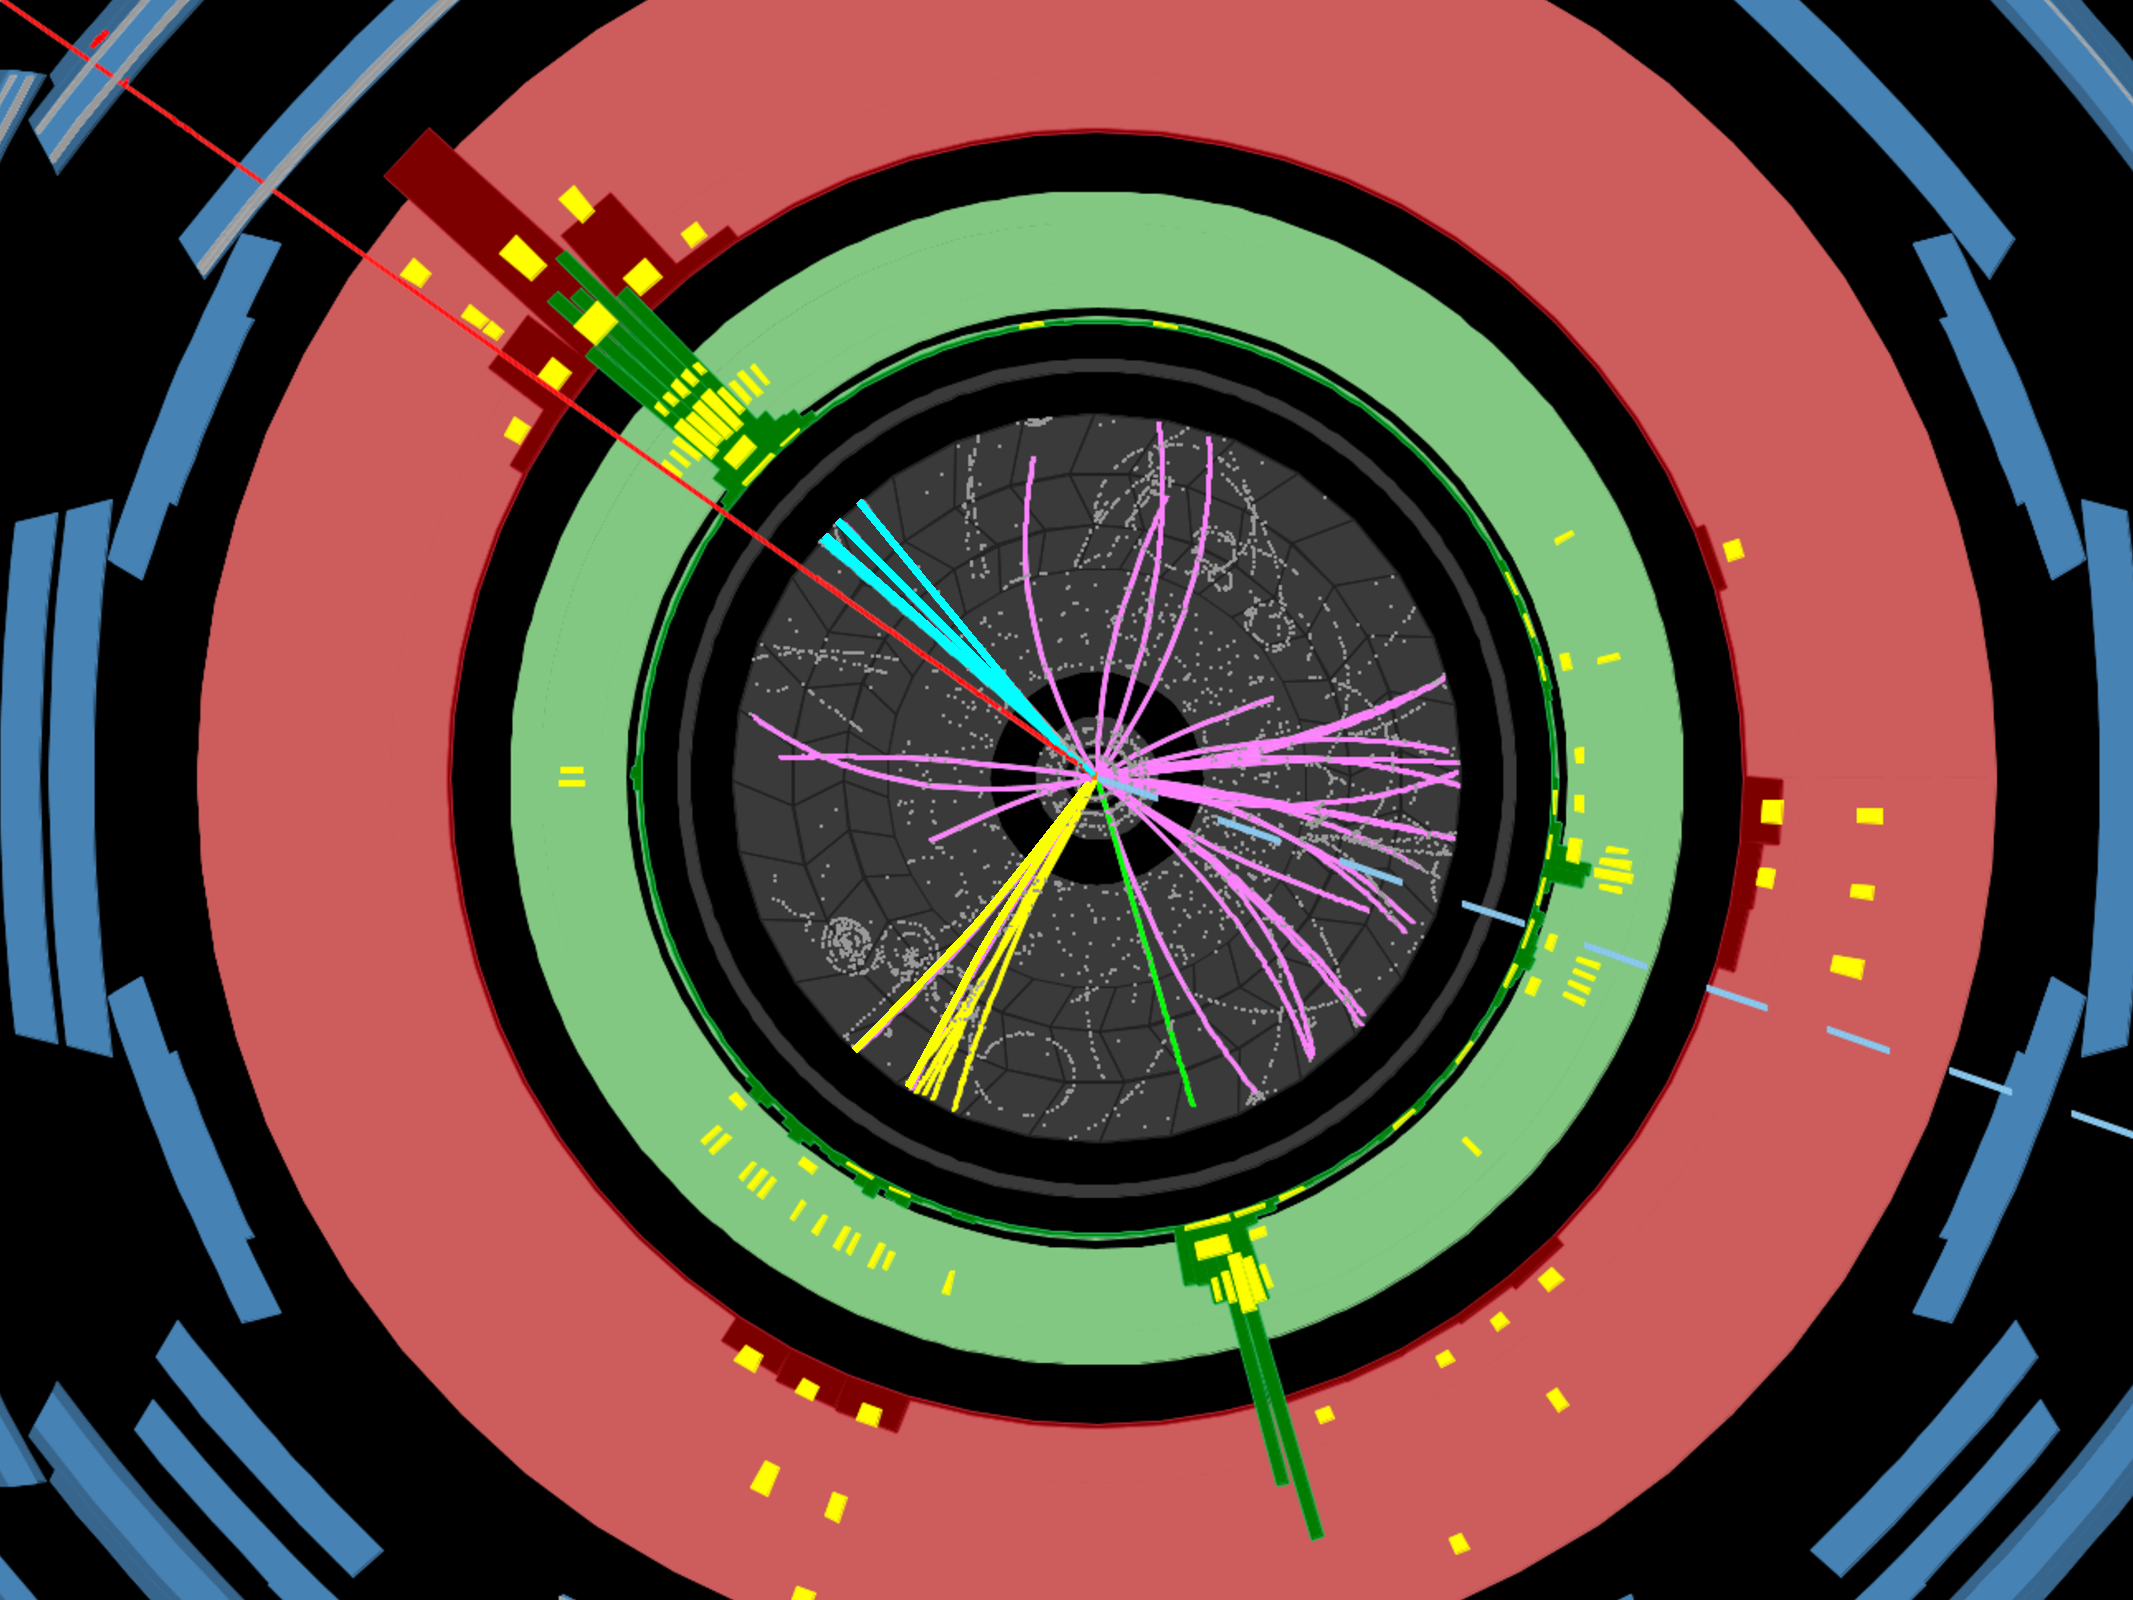
\includegraphics[width=0.8\textwidth]{./EventDisplayNoLabel.pdf}
\ec

\clearpage

There are four basic types of images that the detectors capture. 
You can think of these as the basic outputs of the detectors. 
(Of course this is not the true output of the detectors which really just measure voltage or charge, but it is a convenient abstraction and its the level at which most experimental HEP physicists think)

This basic outputs are shown below.
Correlations among these four basic image types, tell us what kind of particles where produced in the collision.

\bc
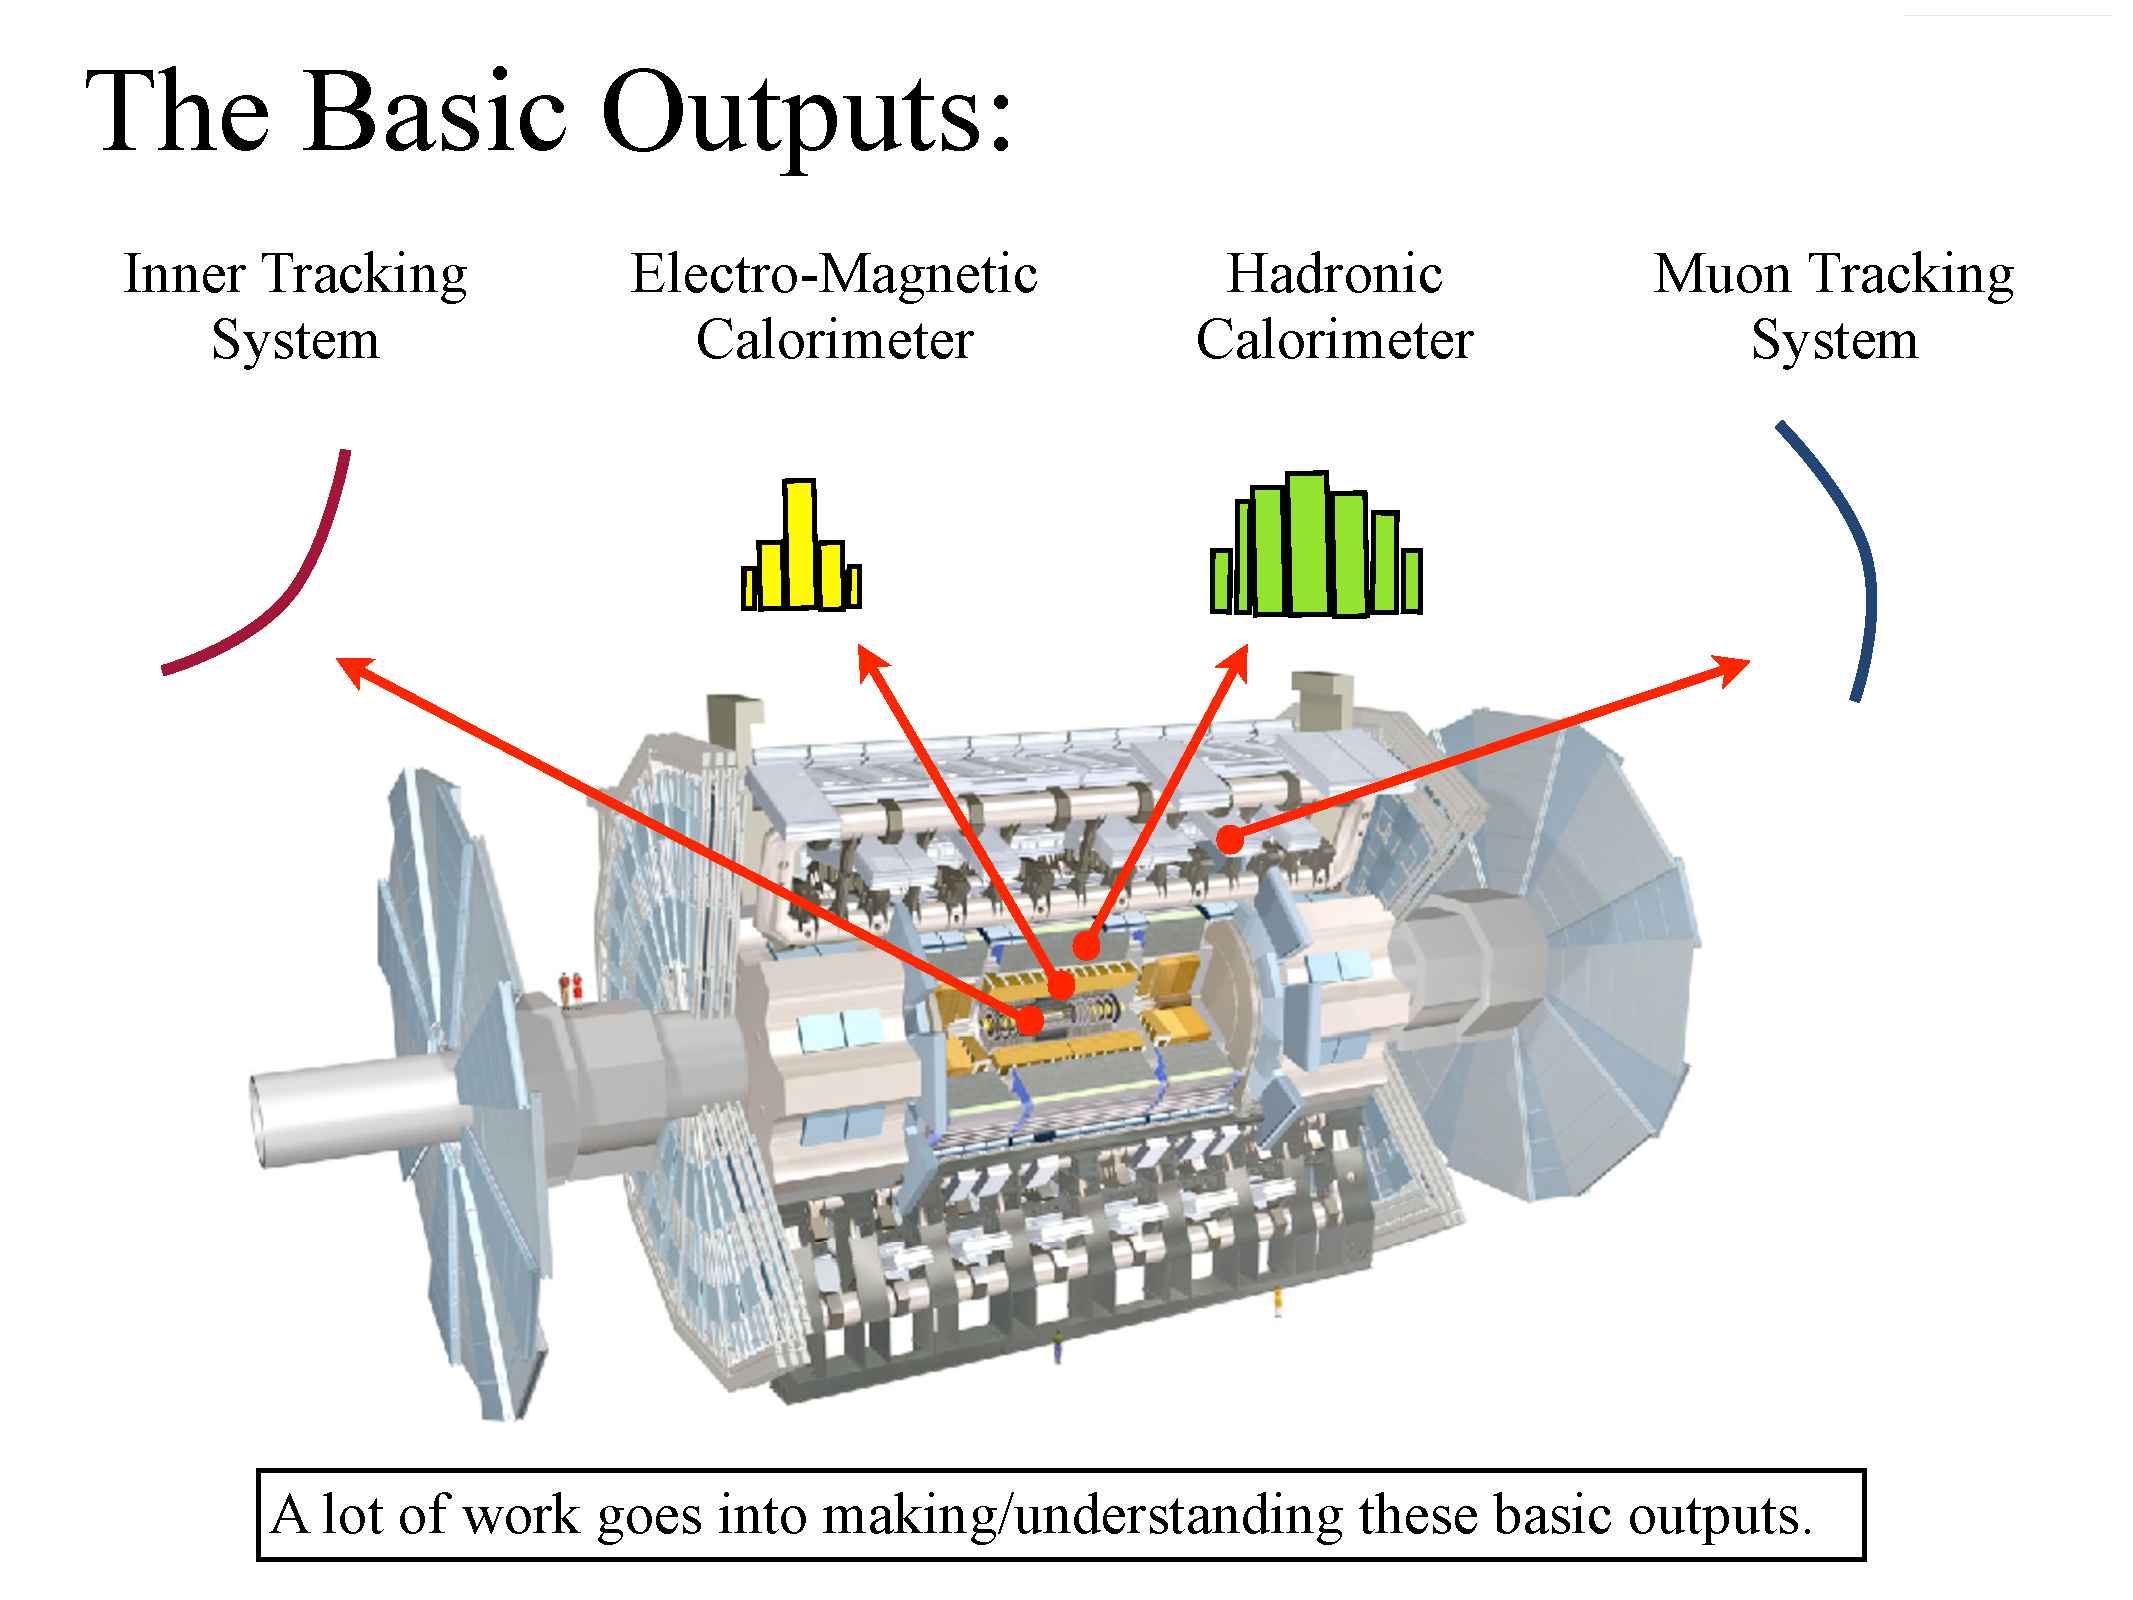
\includegraphics[width=1.0\textwidth]{./BasicInputs.pdf}
\ec

\clearpage

Of course we are really interested in the particles,  not the different image types. 

The particles that exist again are 

\underline{Fermions}
\be
\begin{pmatrix} \nu_e \\ e \end{pmatrix} \hspace*{0.1in} \begin{pmatrix} \nu_\mu \\ \mu \end{pmatrix} \hspace*{0.1in}  \begin{pmatrix} \nu_\tau \\ \tau \end{pmatrix}  \hspace*{1in}  \begin{pmatrix} u \\ d \end{pmatrix} \hspace*{0.1in}   \begin{pmatrix} c \\ s \end{pmatrix} \hspace*{0.1in}   \begin{pmatrix} t \\ b \end{pmatrix}  \times \rmt{3 colors}
\ee

\underline{Bosons}
\be
g \times \rmt{8 colors}  \hspace*{0.2in} W^\pm  \hspace*{0.2in} Z  \hspace*{0.2in} \gamma    \hspace*{0.2in} H
\ee

\lineacross

Experimentally, 

\bi
\item[-] $e$, $\mu$ and $\gamma$, are easy to identify 
\item[-] $\nu_e, \nu_\mu, \nu_\tau$ all look alike, but distinct from other at high \pt.  (Can only tell if at least one is present) 
\item[-] $\tau$ hard but possible (some $\tau$s decay to $e$s or $\mu$s)
\item[-] $u,d,s,c,b,g$ all look alike, bs can be separated 
\item[-] Heavy particles decay into combination of above signatures: Use QFT to calculate how and with what probability this occurs 
\ei

But by correlation the three basic images we can infer which particles were present. 
How this is done for the fermions is shown here:
\bc
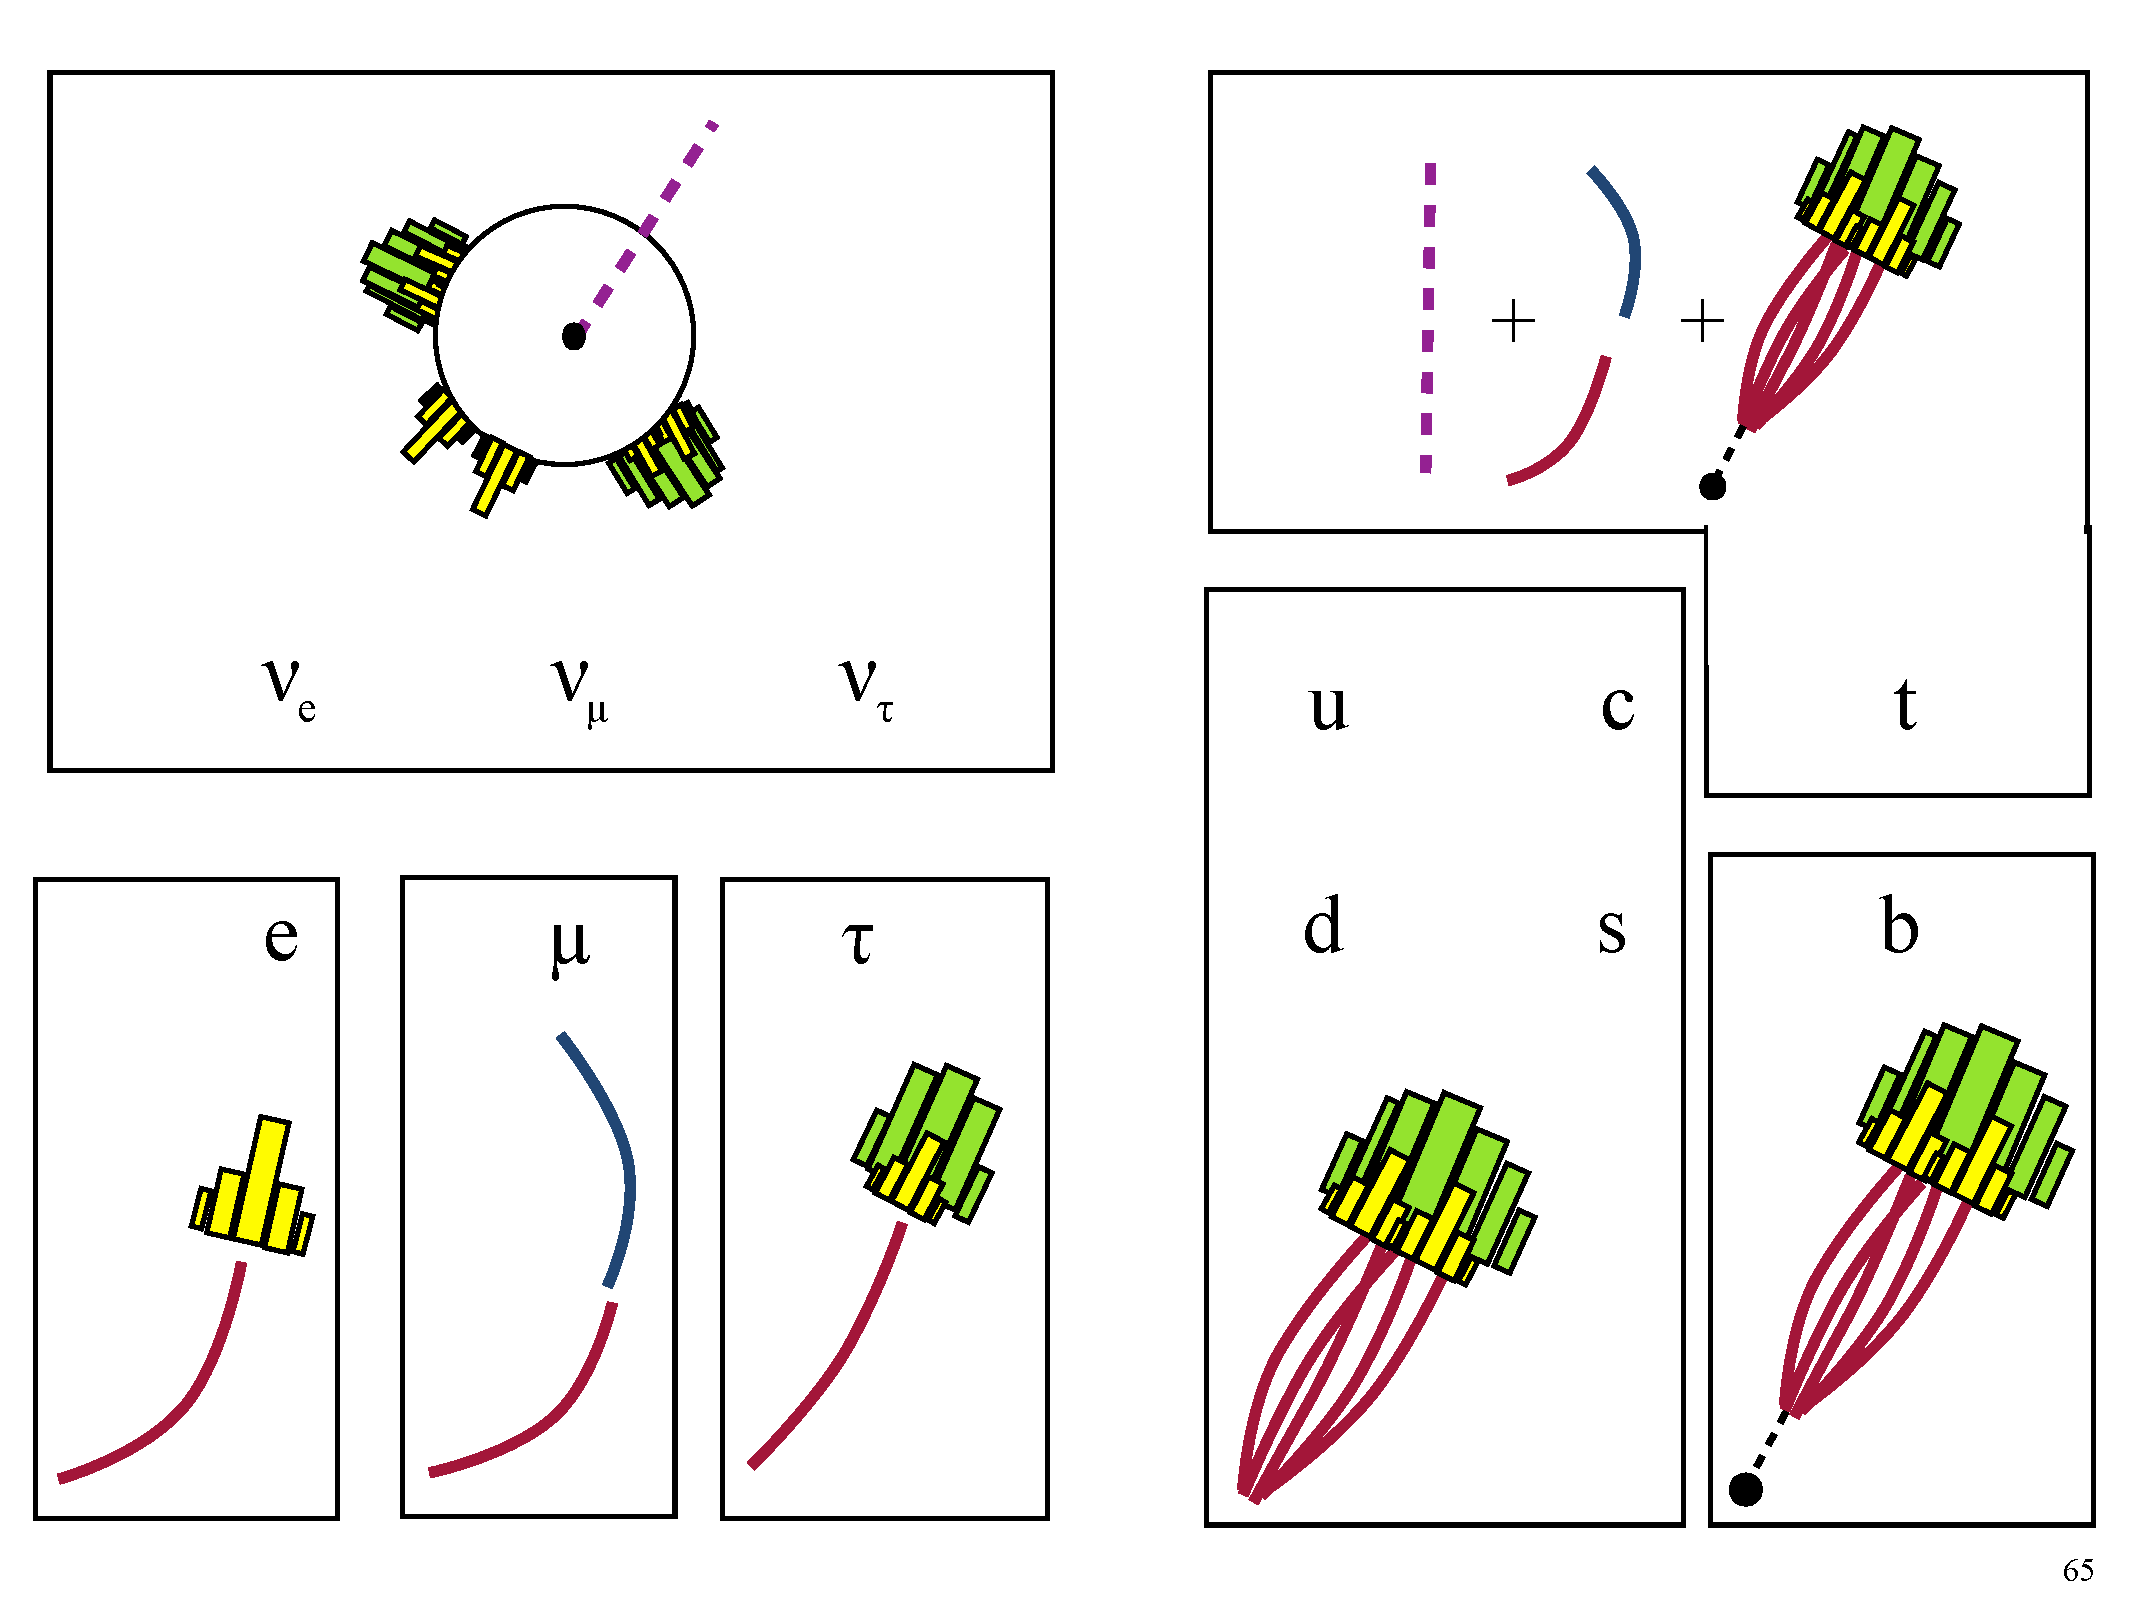
\includegraphics[width=0.5\textwidth]{./Fermions.pdf}
\ec

\clearpage
The detector signature of the Bosons is:
\bc
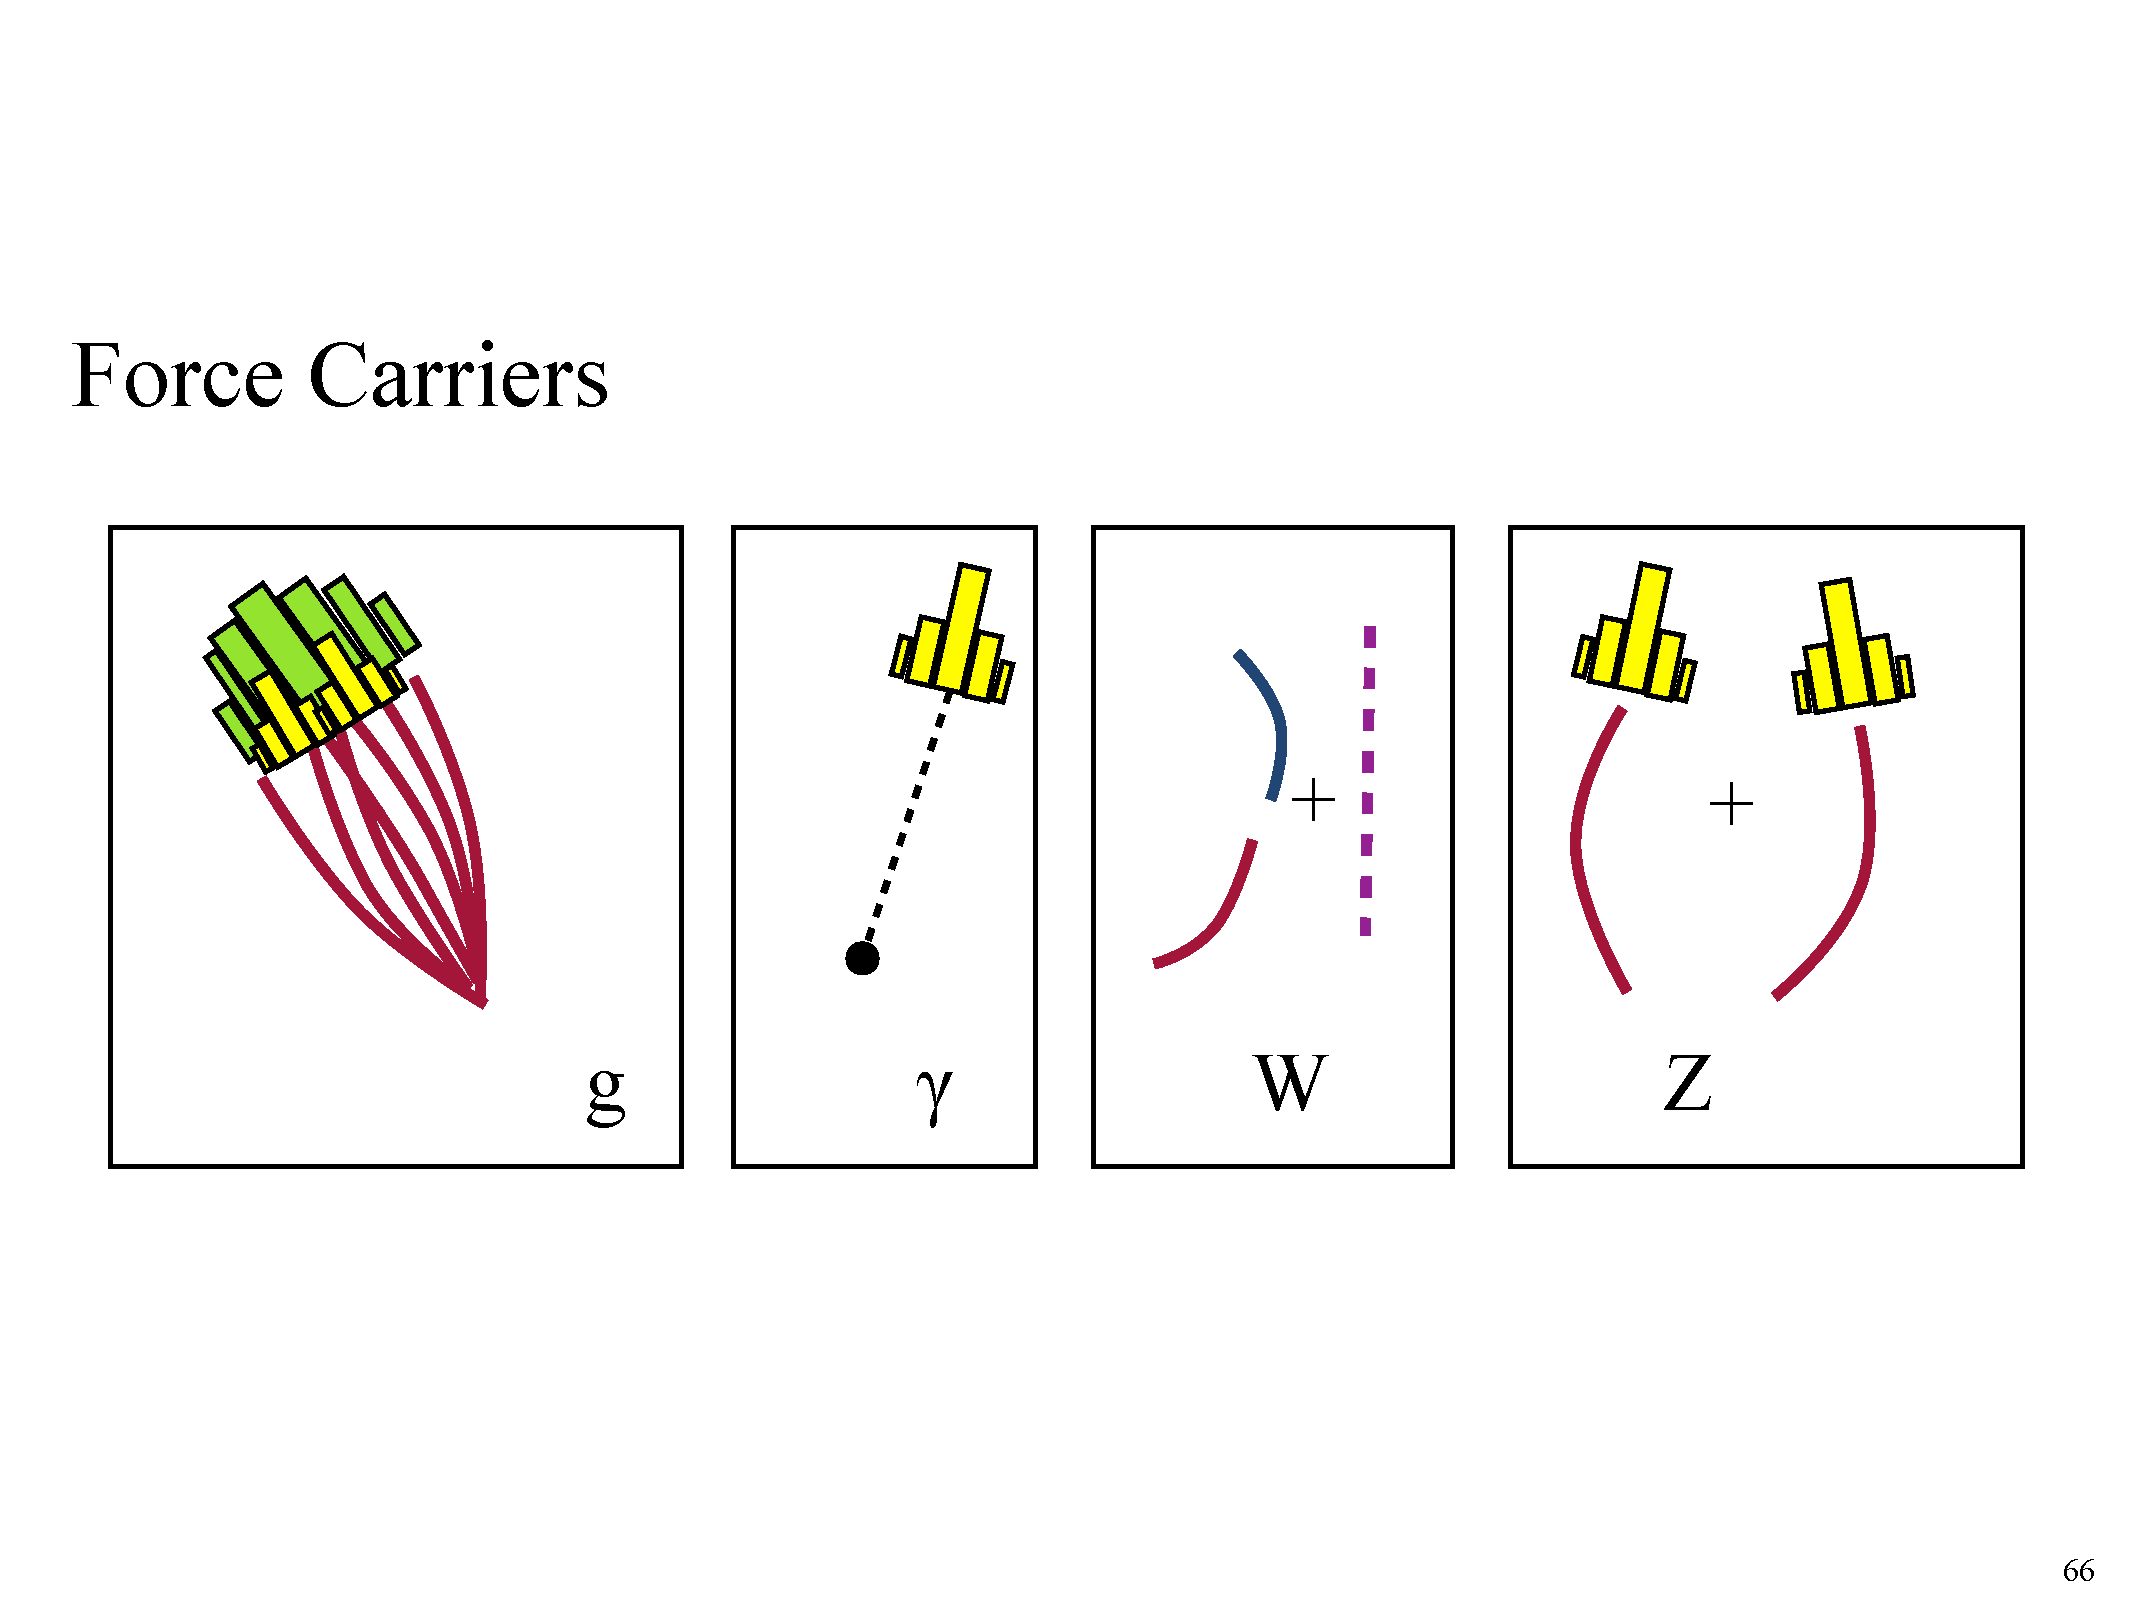
\includegraphics[width=0.75\textwidth]{./Bosons.pdf}
\ec
\bc
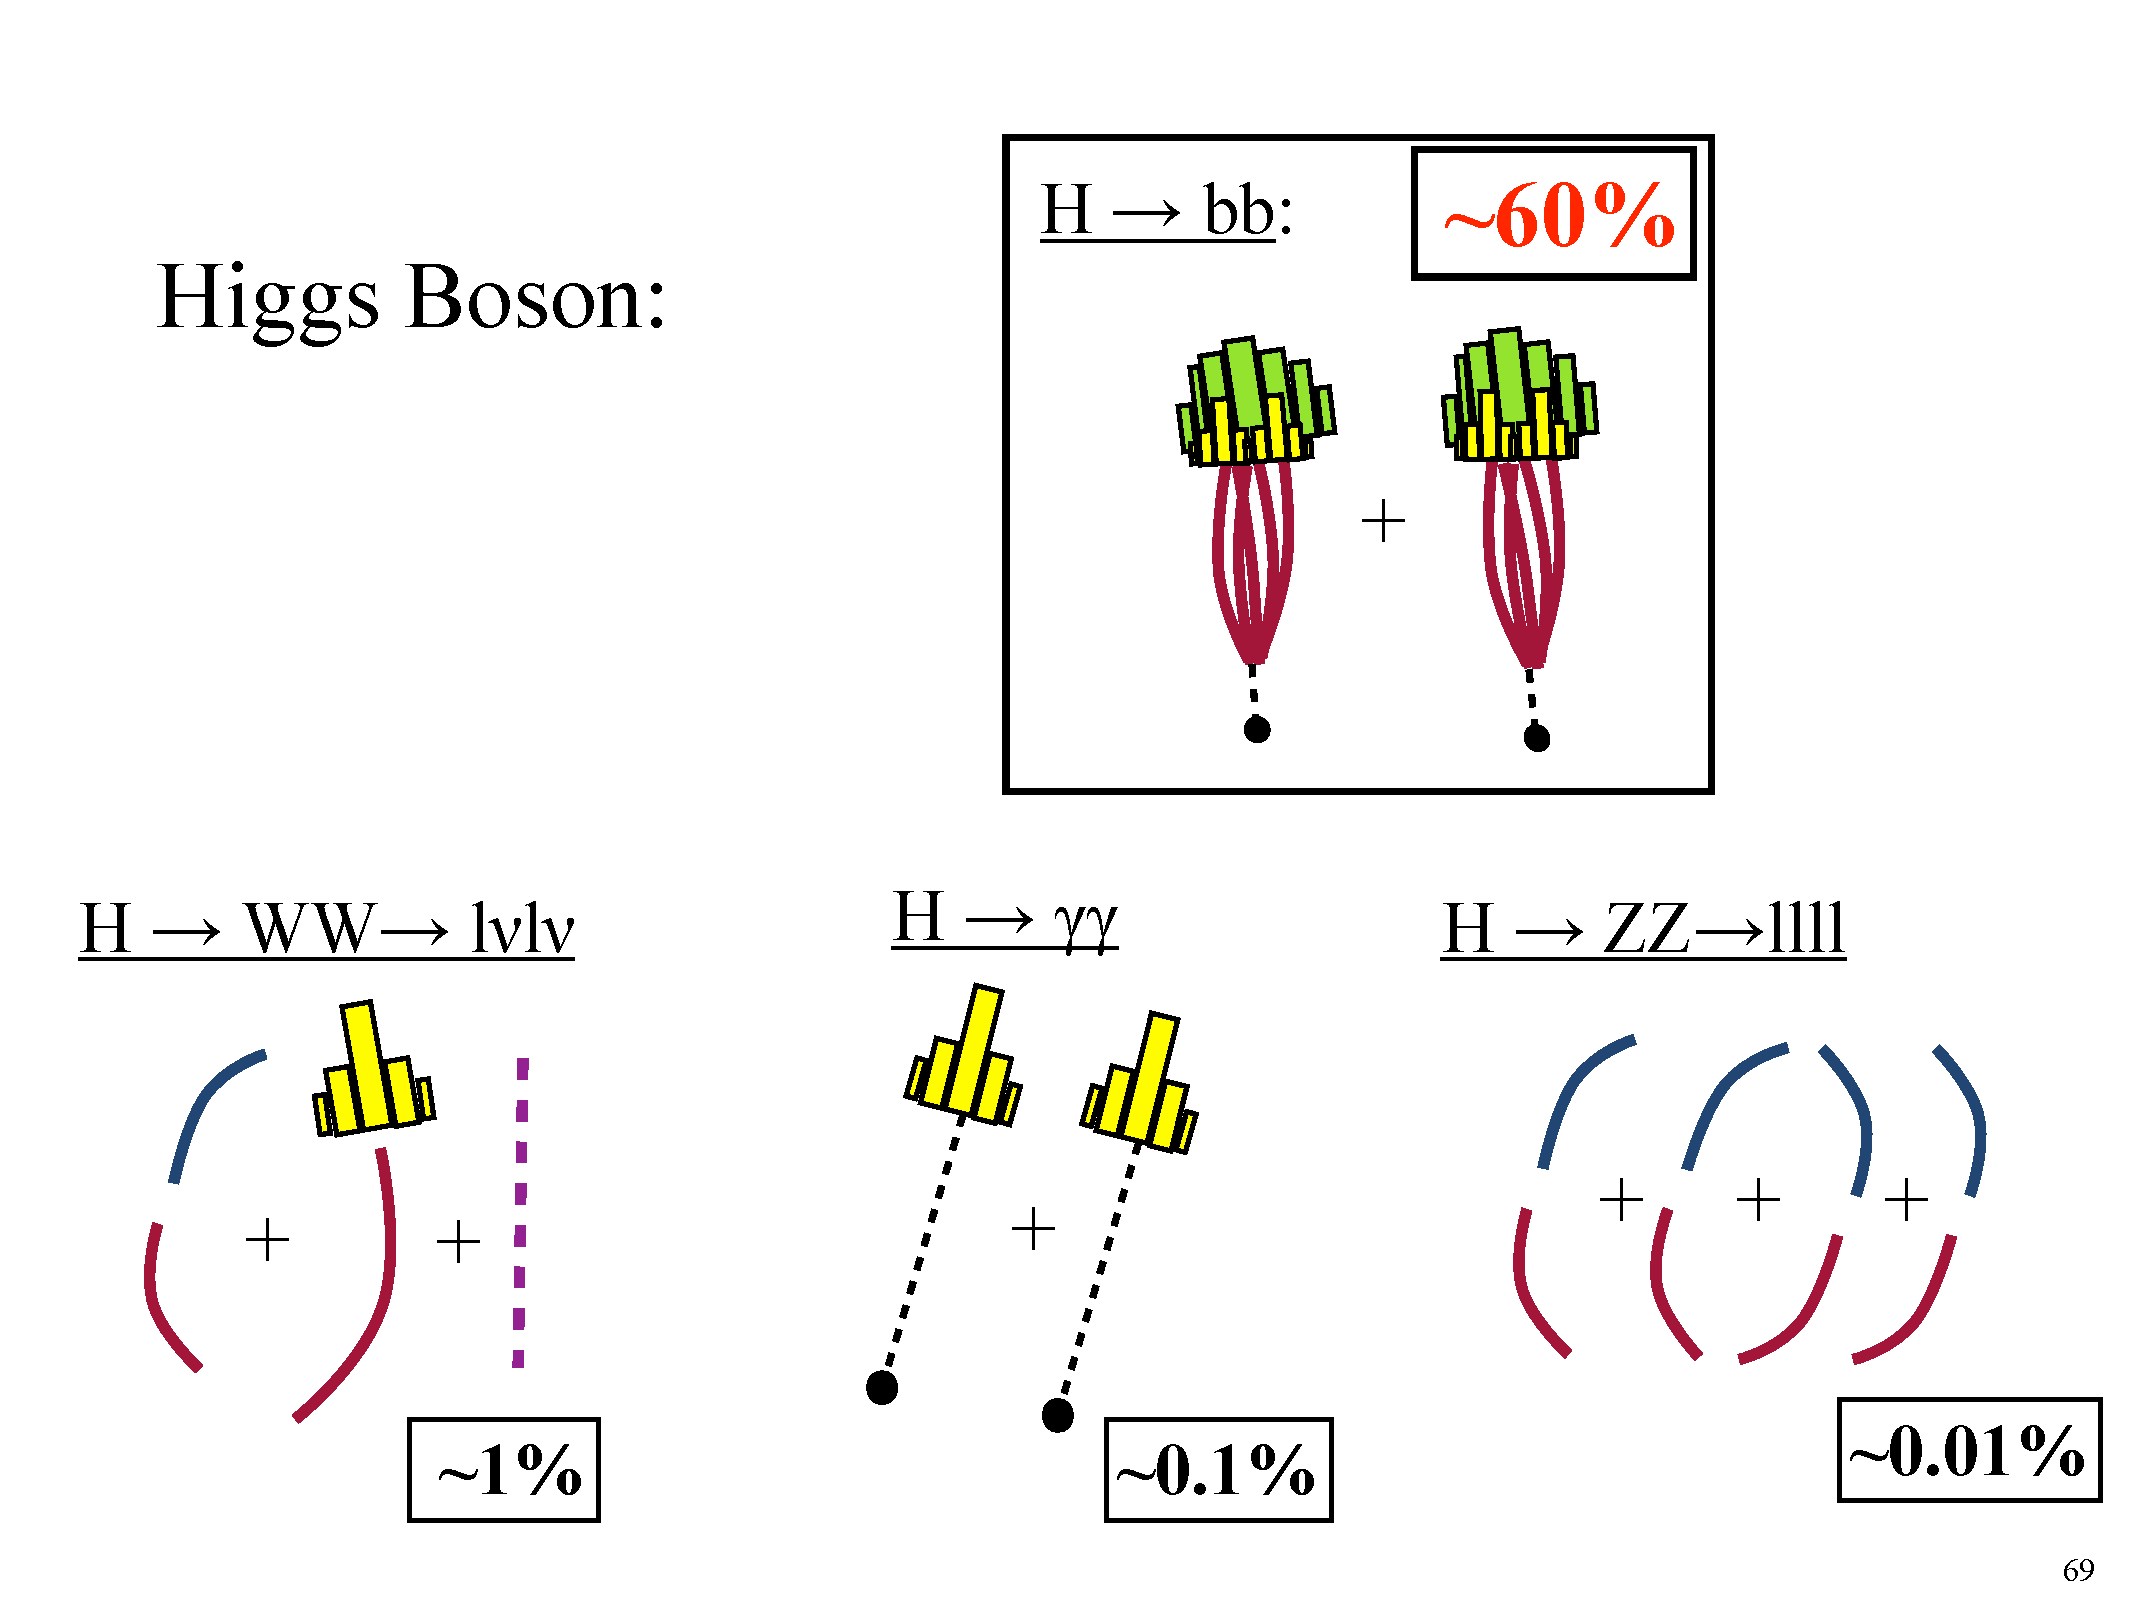
\includegraphics[width=0.75\textwidth]{./HiggsBoson.pdf}
\ec

\clearpage
Often interested in how particles decay to classes of particles 

\bi
\item[-] $l^\pm$s $\{e, \mu, \tau\}$
\item[-] $\nu$s
\item[-] b-jets
\item[-] ``jets''  $\{u,d,s,c,b,g\}$
\ei

-) Probability to decay is given by 

\be
\Gamma = \frac{1}{2E_p} |M|^2 d\Pi_{LIPS}
\ee


\begin{minipage}{0.6\textwidth}
-) The relative probabilities dictates how often a particle decays a certain way: 
\end{minipage} \hfill
\begin{minipage}{0.3\textwidth}
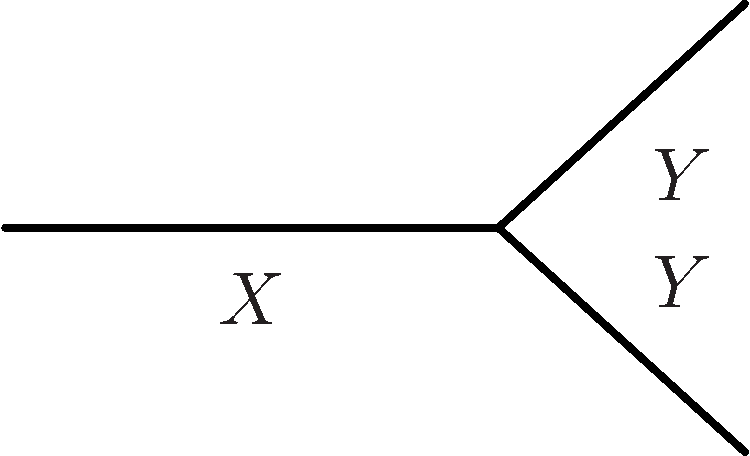
\includegraphics[width=0.8\textwidth]{./XToYY.pdf}
\end{minipage} 

$Br(X\rightarrow YY)$ probability for particle $X$ to decay to $YY$.

\bea
\underbrace{Br(X\rightarrow YY)}_{\rmt{``Branching \multiline{Ratio'' \\ Fraction''}}}  &=&  \underbrace{\frac{\Gamma(X\rightarrow YY)}{\sum_f \Gamma(X\rightarrow ff)}}_{\sum_f \rmt{Includes all possibilities}} = \frac{ \frac{1}{2E_p}  d\Pi_{LIPS} |M(X\rightarrow YY)|^2}{ \frac{1}{2E_p}  d\Pi_{LIPS}  \sum_f |M(X\rightarrow ff)|^2} \\
&=& \underbrace{\frac{  |M(X\rightarrow YY)|^2}{\sum_f |M(X\rightarrow ff)|^2} }_{m_f, m_Y << m_X}
\eea


Where, $M(X\rightarrow ff)$ is given by the $X\rightarrow ff$ Feynman diagram squared. 

Usually have simple relationships among the M's
(Where the practical QFT comes in...)

\clearpage

\underline{Example 1)}

How often does a Z decay to $e^+e^-$ ?

\bea
Br(Z\rightarrow ee)  &=&  \frac{\Gamma(Z\rightarrow ee)}{\sum_f \Gamma(Z\rightarrow ff)}  \underbrace{=}_{\rmt{Assume Universal Coupling}} \frac{  |M_0|^2}{   \sum_f |M_0|^2}  = \frac{1}{21}\\
&=& \underbrace{\frac{1}{6 + 3 \times 5}}_{\multiline{$6 = \{e,\mu,\tau,3\nu\} + $ \\ 3 colors $\times$ 5 light quarks}}
\eea

Note: $2\times m_{top} > m_Z$ 


\underline{Example 2)}

\be
Br(Z\rightarrow bb)  =   \frac{3 |M_0|^2}{   \sum_f |M_0|^2}  = \frac{3}{21}
\ee


\clearpage

\underline{Example 3)}

$\tau$-decays

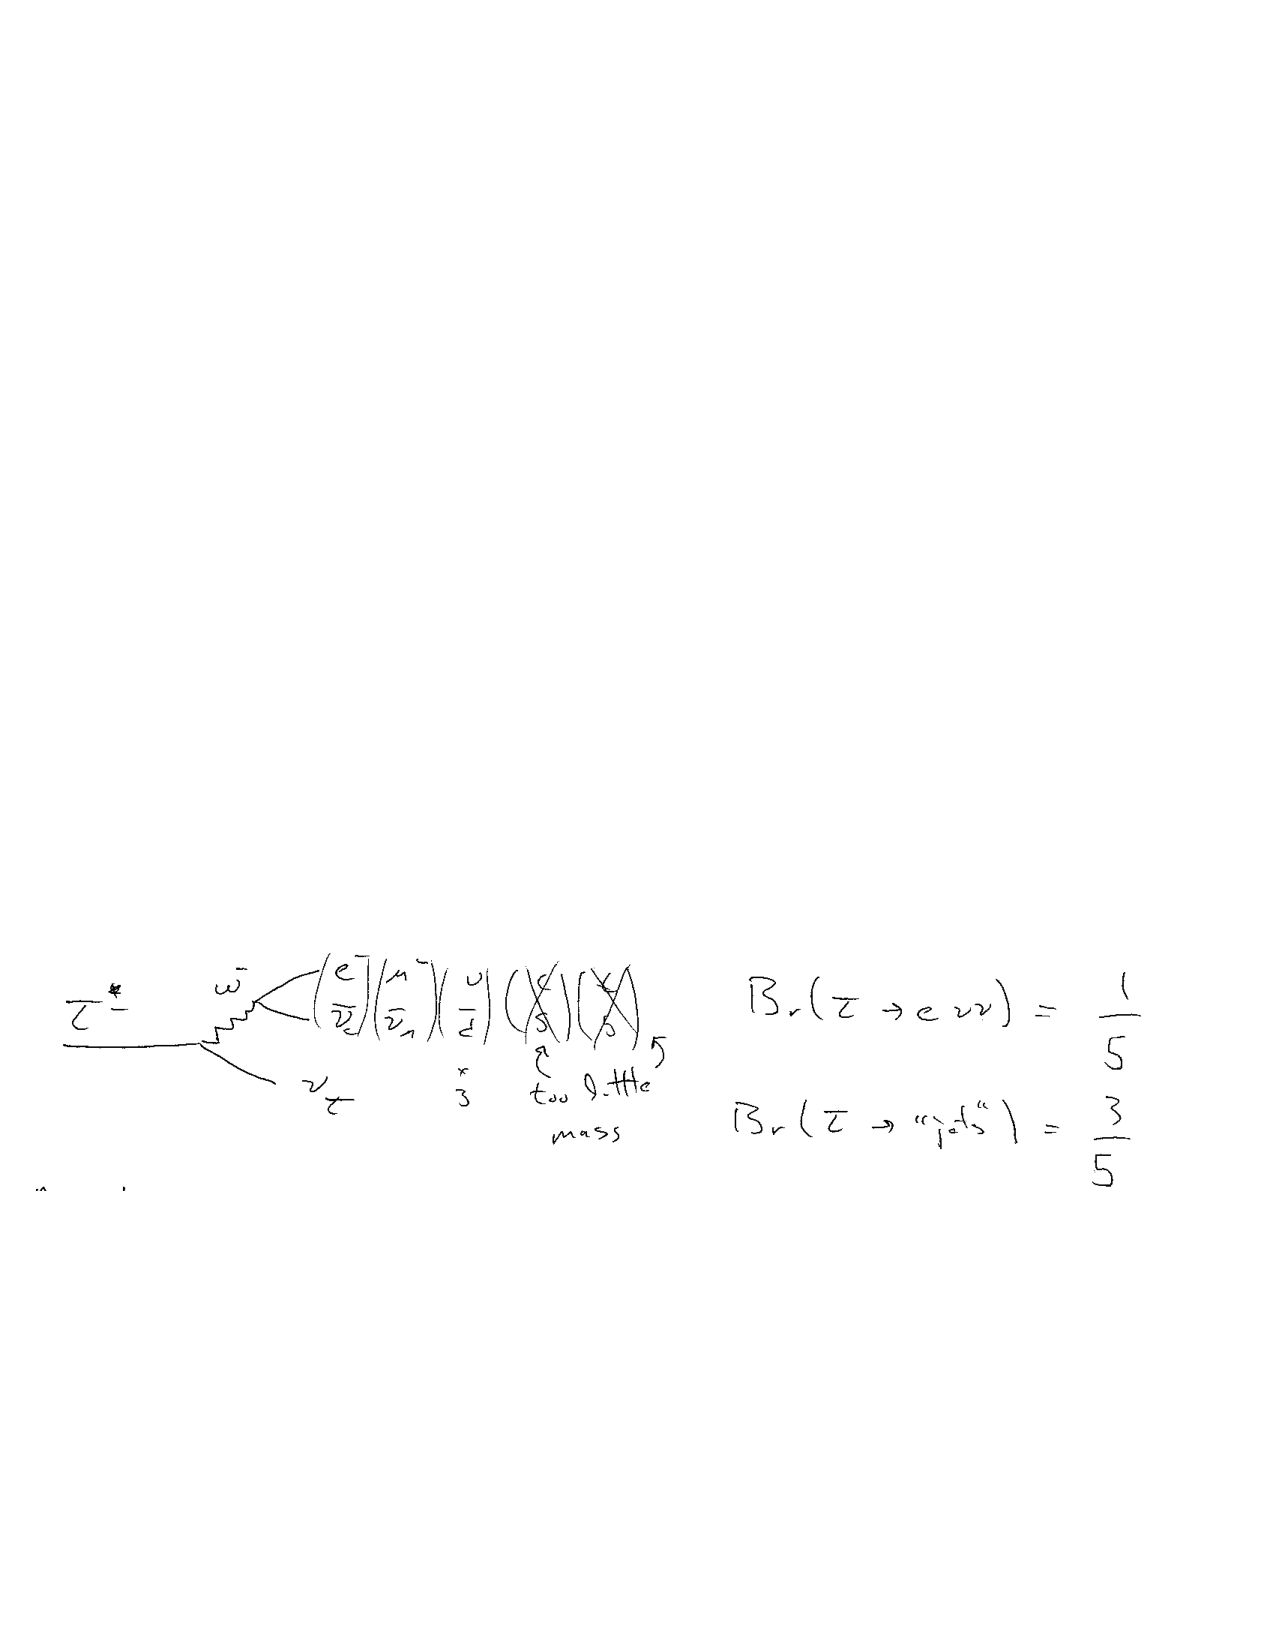
\includegraphics[width=1.0\textwidth]{./tauDecays.pdf}

\vspace*{1in}

\fbox{\begin{minipage}{\textwidth}
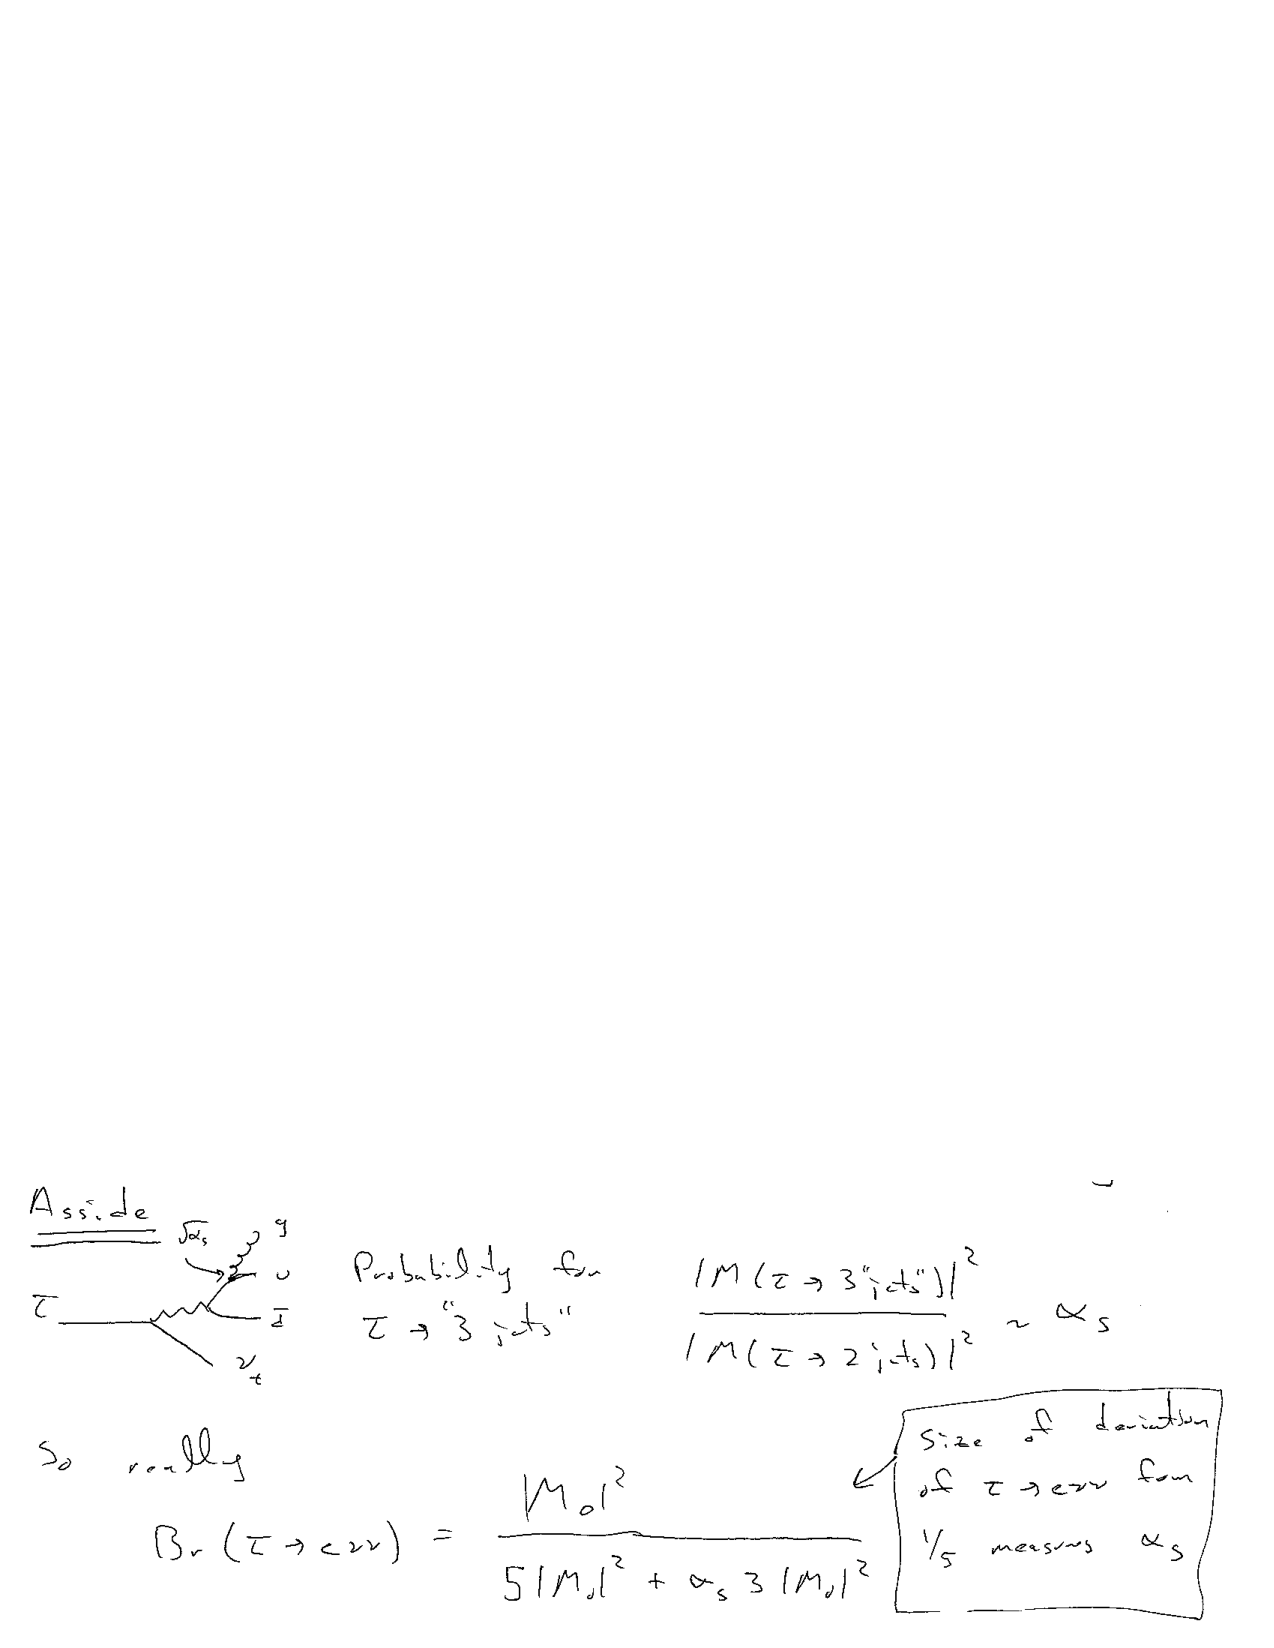
\includegraphics[width=1.0\textwidth]{./alphaSFromTaus.pdf}
\end{minipage}}

}
\end{document}


